\chapter{Design and Implementation}\label{ch:design-implementation}
In this chapter we overview the design of {\sys} traffic shaping tunnel. 


\section{DP Traffic Shaping Simulator}\label{s}
We design and implement a traffic shaping simulator to evaluate the bandwidth overhead and privacy guarantees of {\sys} differentially private traffic shaping mechanism.
The simulator helps the users to configure parameters of {\sys} shaping mechanism, balancing the trade-offs between privacy and overhead according to their requirement.
Then, they can use optimal parameters in the actual {\sys} system.



\section{Traffic Shaping Tunnel}\label{sec:tunnel-overview}

The previous section describes an abstract differentially private traffic shaping strategy.
We now present \sys's traffic-shaping tunnel.

A tunnel must address three requirements. First, it must satisfy DP guarantees. For this, the tunnel~must complete DP measurements and prepare shaped packets within each interval, and it must be able to transmit all payload bytes generated from an application within a finite window length (as defined in the DP strategy).
%
Secondly, the payload and dummy bytes in the shaped packets must be indistinguishable to an adversary.
For this, the payload and dummy bytes must be transmitted through a shared transport layer so that they are identically acknowledged by the receiver and subject to congestion control and loss recovery mechanisms.
%
Finally, the tunnel must provide similar levels of reliability, congestion control, and loss recovery as expected by the application.
\begin{figure}[t]
  \centering
  %  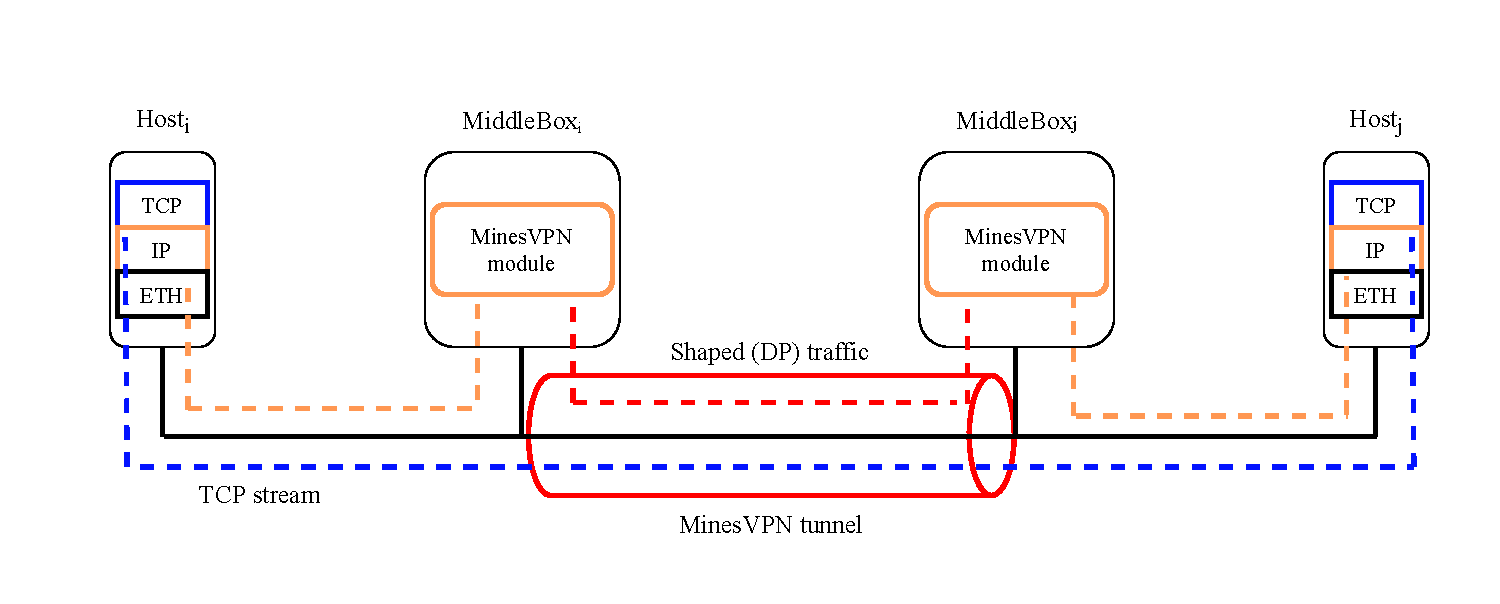
\includegraphics[width=\columnwidth]{figures/Design_highlevel.pdf}
  %  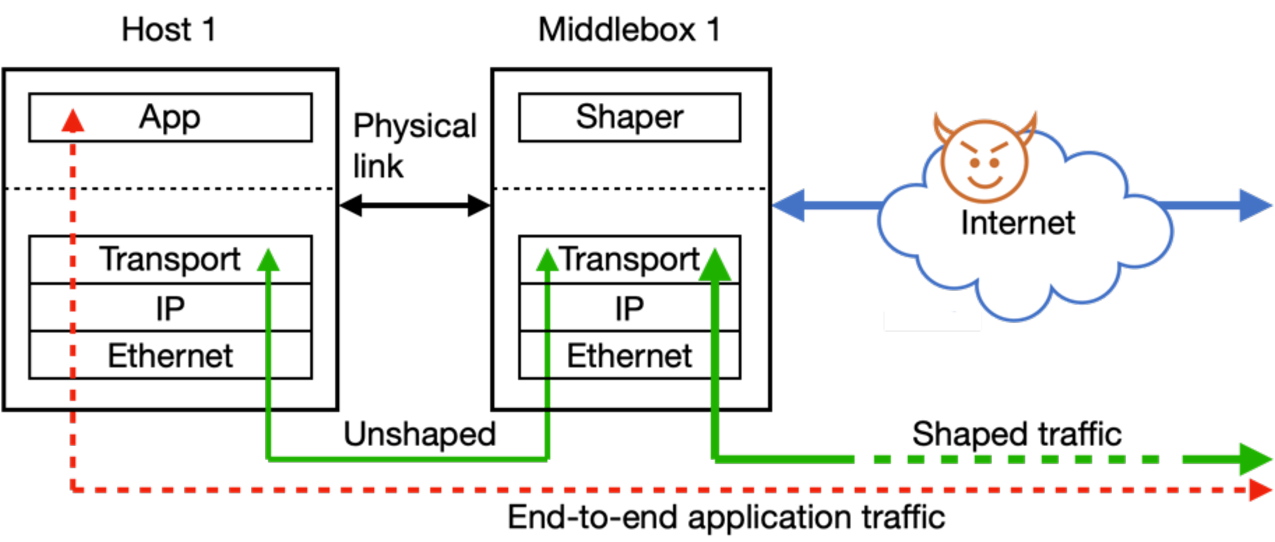
\includegraphics[width=\columnwidth]{figures/minesvpn-overview-half.pdf}
  %  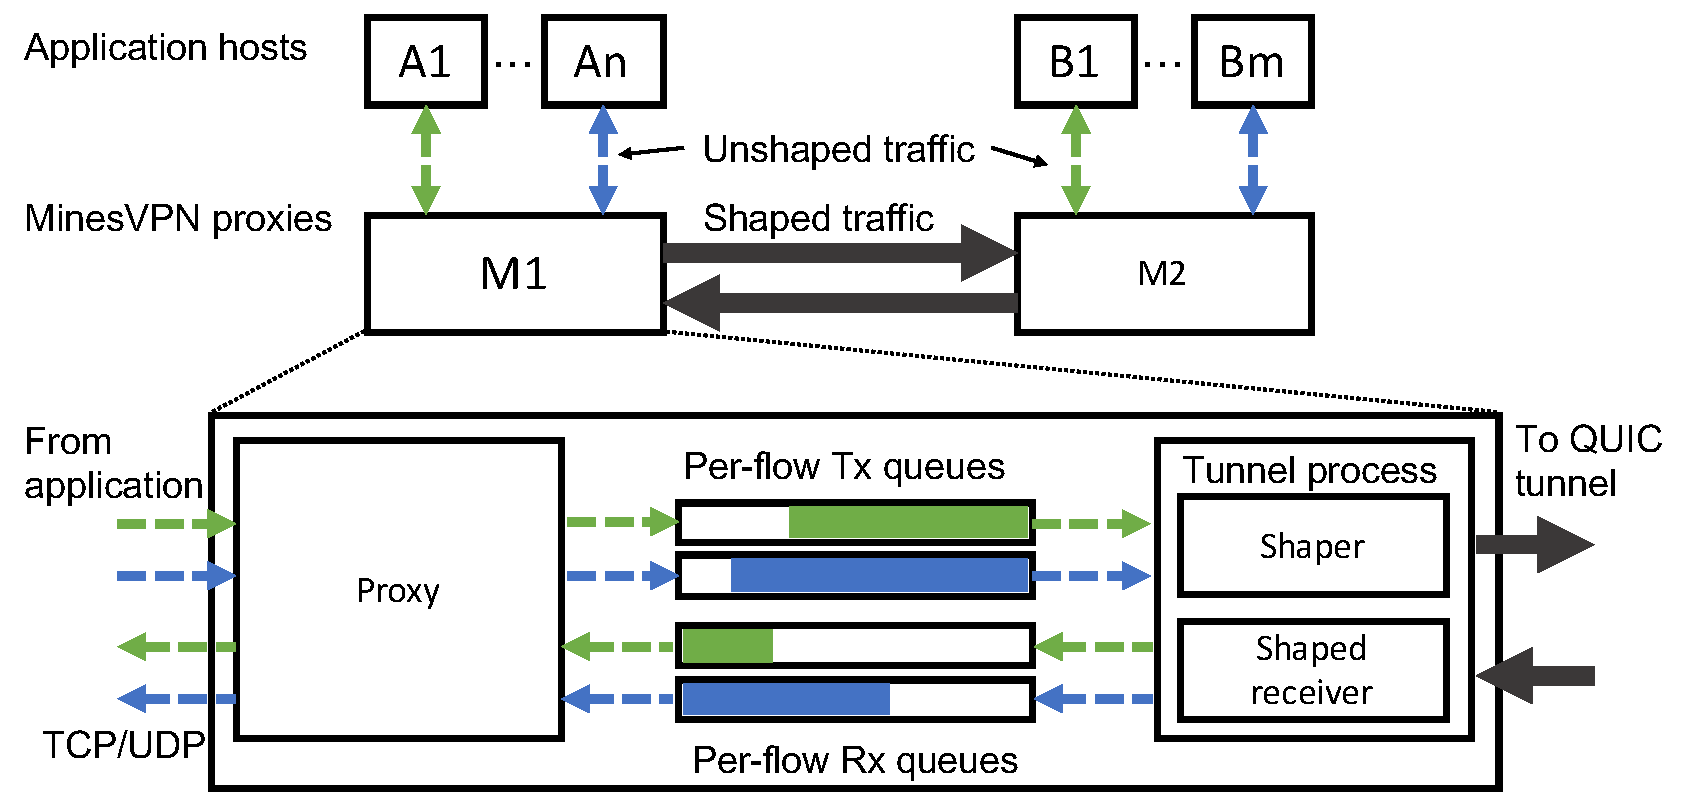
\includegraphics[width=\columnwidth]{figures/minesvpn-arch4.pdf}
  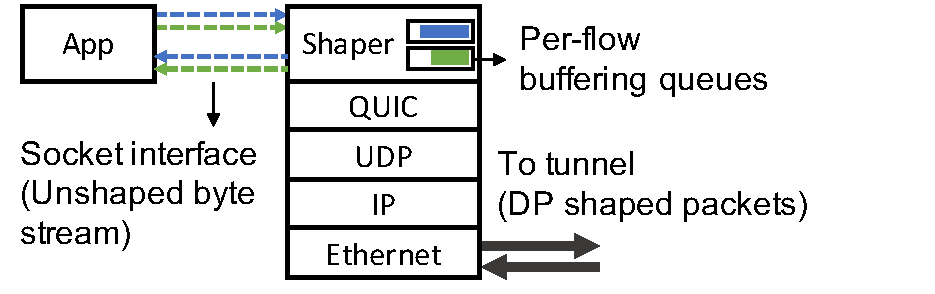
\includegraphics[width=\columnwidth]{figures/design2.pdf}
  \caption{Overview of tunnel design (one endpoint)
      %\am{Update figure}
  }
  \label{fig:minesvpn-overview}
\end{figure}

\Cref{fig:minesvpn-overview} shows the design of one endpoint of {\sys}’s traffic shaping tunnel. A similar endpoint is deployed on the other end of the tunnel.
The shape of the traffic in the tunnel can be configured independently in each direction. The privacy loss in bidirectional streams is the DP composition of the privacy loss in each direction.
A tunnel endpoint consists of a shaping layer (Shaper) on top of QUIC, which in turn runs on top of a standard UDP stack
It's worth mentioning that aside from QUIC/UDP, {\sys} has the option to utilize a conventional TCP stack as well.
The tunnel endpoints establish a bidirectional QUIC connection and generate DP-sized transmit buffers in fixed intervals, which carry payload bytes from one or more application flows.
In the absence of application payload, a tunnel endpoint transmits dummy bytes, which are discarded at the other endpoint.
QUIC encrypts all outbound packets.

{\sys} adopts a transport-layer proxy architecture: each application terminates a connection with its local tunnel endpoint.
The application byte stream is sent to the remote application over three piecewise connections: 
(i) between the application and its local tunnel endpoint,
(ii) between the tunnel endpoints, and
(iii) between the remote tunnel endpoint and the remote application.
This ensures only one active congestion control and reliable delivery mechanism in the tunnel and that all bytes are subject to identical mechanisms.
We discard tunneling TCP through TCP and use QUIC as TCP-in-TCP tunneling causes TCP meltdown~\cite{honda2005tcpovertcp, tcp-meltdown} problem.
In a TCP-in-TCP tunnel, when the network experiences packet loss, the lower-layer TCP initiates packet retransmission to ensure delivery.
However, the upper-layer TCP protocol is unaware of this packet loss and wrongly interprets the increased delay as a sign of a slow network, leading it to decrease the transmission rate.
Consequently, this slower transmission causes the lower-layer TCP protocol to receive acknowledgments too slowly, further mistaking it as packet loss within the network, and thus triggering retransmission.
This repetitive cycle creates a detrimental effect on network performance known as the TCP meltdown problem, significantly degrading overall efficiency.
The other option was to use TCP-in-UDP tunnel. 
This, however, violates the privacy guarantees of {\sys}.
In case of packet losses, the application TCP protocol retransmits data to guarantee data delivery. 
On the other hand, the dummy bytes that are injected in the traffic shaping tunnel are not retransmitted, making them observable for adversary. 


\section{Tunnel Design and Operations}\label{sec:tunnel-design}
In this section, we present an overview of the fundamental operations that a well-designed {\sys} tunnel should encompass.
Irrespective of its implementation, a {\sys} tunnel must offer a set of essential functionalities, including tunnel setup and teardown, connection establishment and termination, outbound traffic shaping, and inbound traffic processing. 
In the following subsections, we delve into each of these critical functionalities to provide an understanding of their significance and roles within the system.

\paragraph{Tunnel setup and teardown}
Before applications can communicate with each other, a {\sys} tunnel must be set up between their local tunnel endpoints.
The initiator application sends a configuration message to its local tunnel endpoint with the source and destination IP addresses and ports, a reliability flag, and a privacy descriptor.
The reliability flag indicates if the tunnel should provide reliable delivery semantics or not.
The privacy descriptor indicates the DP parameters to be used for shaping the tunnel traffic.

Upon receiving a configuration message, the Shaper establishes a QUIC connection with the remote tunnel endpoint and configures the reliability semantics and privacy parameters for each direction.
It also initializes three types of bidirectional~streams in the tunnel: control, dummy, and data streams.
One {\em control stream} is used to transmit messages related to the establishment and termination of a connection between the application endpoints. A
{\em dummy stream} transmits dummy in QUIC packets in the form of STREAM frames.
We should note that we do not use QUIC's PADDING frames as they do not elicit acknowledgements and hence are distinguishable from STREAM frames \cite{rfc9000}.
The tunnel pre-configures a finite number of data streams, which carry payload bytes from one or more application flows.
When the tunnel is inactive for a period of time, one of the tunnel endpoints initiates a termination sequence and closes all open QUIC streams and the tunnel connection.

\paragraph{Connection establishment and termination}
Once a tunnel is ready, applications can establish and terminate connections with each other, which is mediated by the tunnel.
When the initiator application runs a connection establishment handshake with its local tunnel endpoint, the Shaper maps the application flow to a per-flow buffering queue and one of the inactive QUIC data streams in the tunnel, and notifies the remote tunnel endpoint.
The remote tunnel endpoint establishes a connection with the receiver application and maps the receiver application's flow with the data stream.
The connection termination handshake is handled similarly by the tunnel endpoints.
The messages for connection establishment and termination are transmitted over the control stream in the tunnel and shaped according to the tunnel's parameters.

\paragraph{Outbound traffic shaping.}
The Shaper accumulates the outbound bytes of an application flow in a buffering queue before it transmits them in packets whose sizes and timing follow a distribution that guarantees DP.
Within a tunnel, the Shaper transmits bytes from all active flows into a differentially-private packet sequence.
At periodic intervals, called DP measurement intervals, it performs a DP measurement on the per-flow queues to determine the number of bytes $\qlendp$ to be~transmitted according to the tunnel's DP parameters.
It prepares a {\em shaped buffer} consisting of $\payload$ payload bytes and $\dummy$ dummy bytes, where $\payload$ is the minimum of $\qlendp$ and the application bytes available in the buffering~queues, and $\dummy = \qlendp - \payload$, which may lie between 0 and $\qlendp$.
The Shaper then passes the buffer with the position and length of the padding to QUIC.

QUIC transforms the shaped buffer into one or more STREAM frames based on the
congestion window, the flow window of the receiver endpoint, and the MTU
(maximum transmission unit).
It places the padding bytes into a dummy STREAM frame.
QUIC packages the frames into packets, whose length is at most MTU minus the length of the headers and whose payload is encrypted.
QUIC forwards the packets to the UDP layer, which subsequently transmits the prepared packets as quickly as it can, given the line rate of the NIC.

{\sys} configures the DP measurement interval such that the Shaper can prepare each shaped buffer within an interval.
If the preparation time for a buffer exceeds the interval, the Shaper discards the buffer.
This ensures that the buffering queue length does not grow significantly, which in turn controls the overhead incurred due to DP shaping.
We evaluate the impact of the length of the buffering queue and the DP
measurement interval on privacy guarantees, bandwidth overheads, and latency
overheads in {\addref}.

\paragraph{Inbound traffic processing.}
A tunnel endpoint receives shaped packets from the tunnel and applies inverse
processing on each packet.
QUIC receives the packet and
sends an ACK to the sender. Subsequently, it decrypts the packet, discards the
dummy frame, and forwards the payload bytes from the remaining STREAM frames to
the application.

